\section{Optimization of Performance}
This section introduces the optimization methods to reduce the latency in the
virtualized systems based-on VMs and Containers.

\subsection{Optimization for VMs}
Gallenmüller et al.\ have shown that measures such as kernel isolation,
disabling virtual cores or disabling energy saving mechanisms and reducing the number of
interrupts can be achieved by modifying parameters in the Linux system\cite{b13}.
Using these mechanisms, the latency of packet-processing Apps can be reduced as low as
\si{25}{$\mu$s} in the worst case.
\begin{figure}[h!]
    \centering
    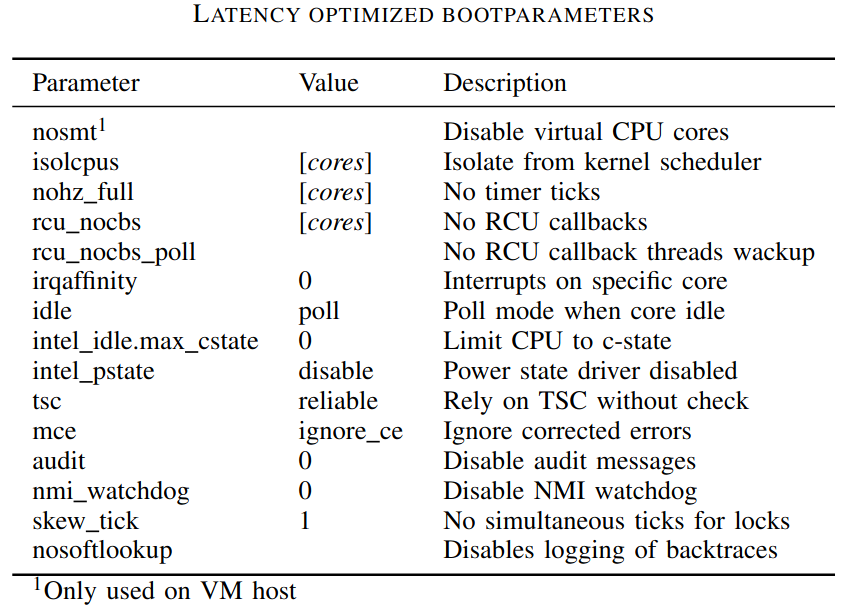
\includegraphics[width=.4\textwidth]{pics/Optimization1.png}
    \caption{Parameter list\cite{b13}}
\end{figure}
During optimization, we can use the parameters in Figure 3.

\subsubsection{Disable Virtual Cores}
Disabling virtual cores can be achieved via the $nosmt$ kernel boot parameter\cite{b13}.
It must be disabled to avoid the effects of unnecessary resource contention between
different virtual cores.

\subsubsection{Enable Core Isolation}
The isolation is enforced by the parameter $isolcpu$ which prevents the Linux scheduler
from scheduling processes to a specific kernel\cite{b13}.
With this configuration, neither the Host OS nor the Guest OS can schedule processes to
the kernel of the executing App.
Therefore, core isolation is achieved which creates the perfect environment for
the uninterrupted execution of packet-processing Apps.

\subsubsection{Reduce the Number of CPU OS Interrupts}
In the research\cite{b10} it was found that not handling OS interrupts that occur on
isolated cores still leads to latency peaks of up to about \si{20}{$\mu$s}.
Therefore, it is necessary to disable scheduling interrupts when running a single App
on a specific core by the parameter $nohz\_full$.
In addition, two option parameters $rcu\_nocbs$ and $rcu\_nocb\_poll$ are needed to
transfer the intra-core read-copy-update processing to different cores, thus avoiding interrupts\cite{b13}.

Furthermore, the NIC can interrupt processing to signal the reception of new packets.
By setting the parameter $irqaffinity$ to 0, data can be processed on the specific core.
The Data Plane Development Kit can also be used to reduce the impact of
the Linux kernel on network Apps in order to achieve high reliability and low latency
on hardware and virtualized systems\cite{b10}.


\subsubsection{Disable Energy Saving Mechanism}
To keep the CPU always in the most active state, the options $idle$
and $intel\_idle.max\_cstate$ can be used.
In addition, $intel\_pstate$ needs to be disabled to prevent the driver from switching the CPU
to a power saving state\cite{b13}.
Disabling the energy saving mechanism improves latency above 99.99\% by about \si{10}{$\mu$s}\cite{b12}.

\subsubsection{Results Based on VMs Latency Optimization}
As shown in the Figure 4, according to the mentioned optimization the network latency of VMs
can be controlled within the limits of the URLLC, when the throughput is less than 80kpkt/s, but it is
still much larger than that of Host.
\begin{figure}[h!]
    \centering
    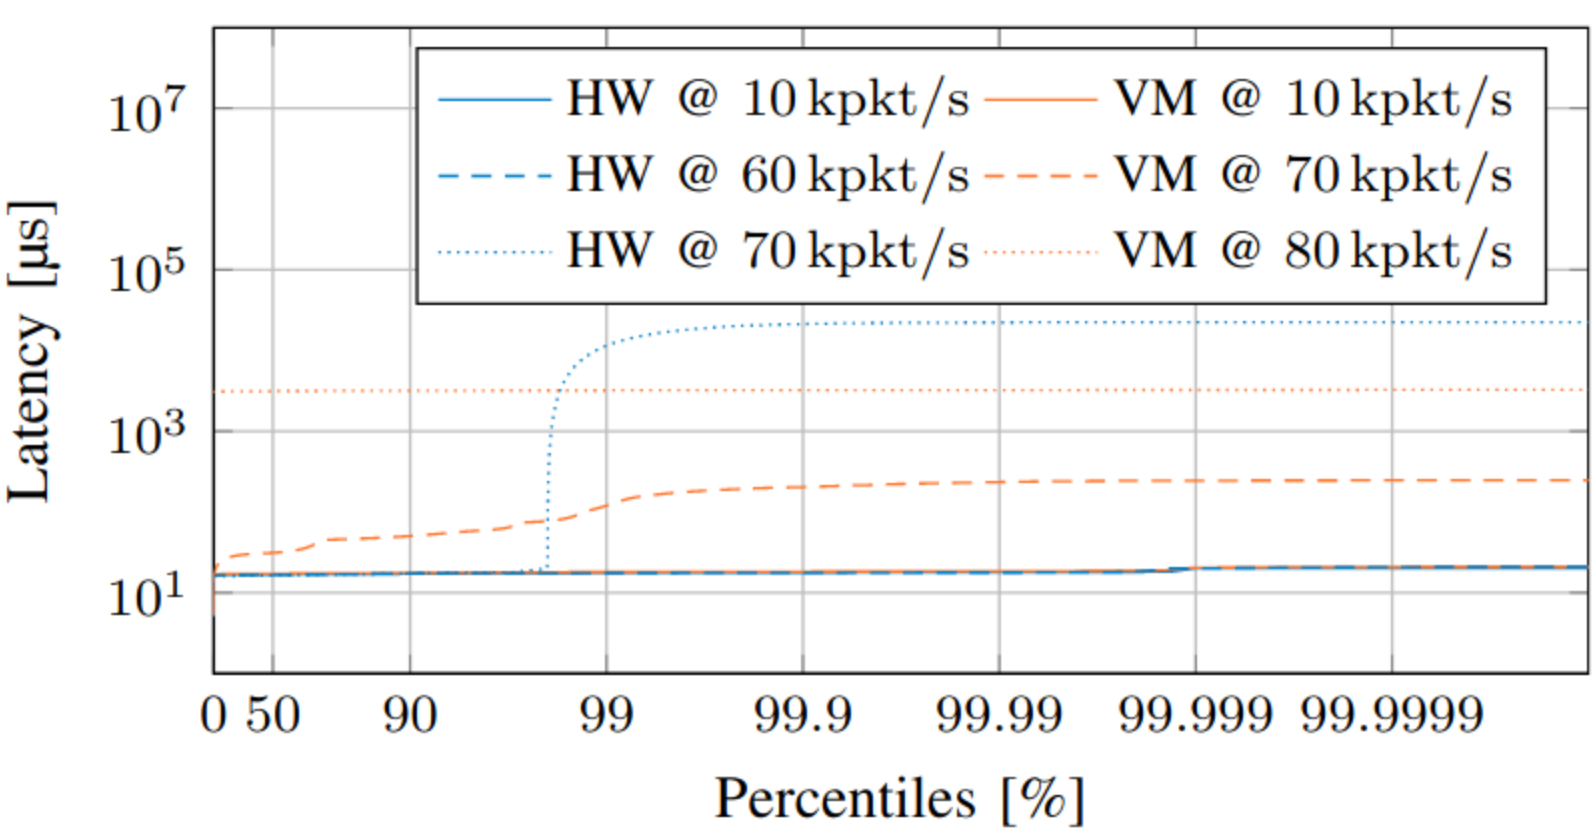
\includegraphics[width=.3\textwidth]{pics/Optimization2}
    \caption{Results based on VMs latency optimization\cite{b13}}
\end{figure}

\subsection{Optimization for Containers}
Different services can be implemented by slicing the network into different
independent logical networks\cite{b10}.
An efficient way to realize network slicing is to share the usage of network resources
among clients.
The small size and high portability of containers meet the demand for deploying numerous
microservices.

\subsubsection{Containers Instead of VMs}
Ann Mary Joy has found\cite{b15}, in the same configuration environment
Docker containers are able to process more requests in the same amount of time.
As shown in the Figure 5, it is 5 times more than VMs, so containers take
less time to process a single request.
In addition, containers take far less time to scale and process service requests than VMs do.
As shown in the Figure 6, the scalability of containers is about 22 times of VMs. Even in
extreme cases, e.g. a container crashes during operation, which affects the performance
of other containers, their performance is still much better than VMs\cite{b7}.

According to Figure 7, it can be seen that the network delay of various container-based
virtualized systems is under 250 {$\mu$s}, which is far lower than the limit of URLLC ($\si{1}{ms}$).

\begin{figure}[h!]
    \centering
    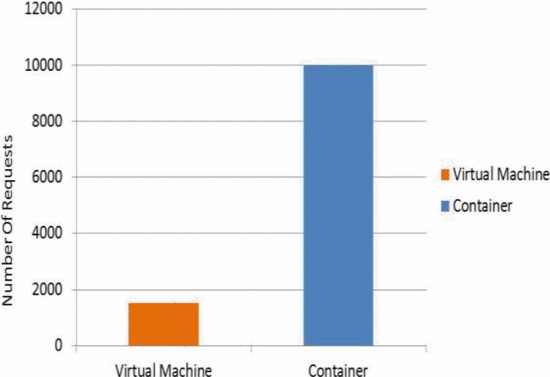
\includegraphics[width=.3\textwidth]{pics/Optimization3}
    \caption{Processing capacity\cite{b15}}
\end{figure}

\begin{figure}[h!]
    \centering
    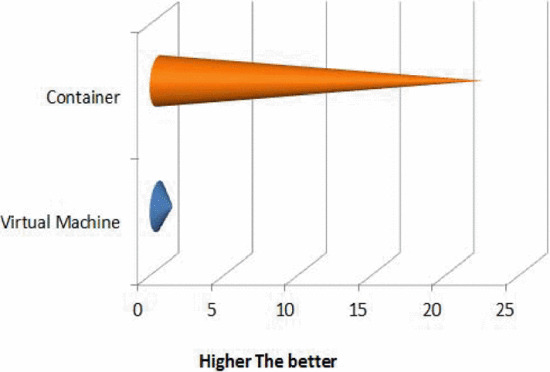
\includegraphics[width=.3\textwidth]{pics/Optimization4}
    \caption{Scalability\cite{b15}}
\end{figure}

\subsubsection{Choosing a Lightweight Container}
Figure 7 shows the comparison of network latency among different typical
virtualized containers. People can see, the smaller the packet, the smaller the slope of the latency increase.
The Linux-VServer has near-native latency.
When the data packet is less than 1KB, the network latency is around 50{$\mu$s}.
This is followed by LXC and OpenVZ. The network latency is around 70{$\mu$s}.
The worst results were observed in Xen with a latency of around 100{$\mu$s}.

These results can be interpreted as different implementations of network
isolation for virtualized systems. While Linux-VServer does not implement
virtualized network devices, both OpenVZ and LXC implement network namespaces
that provide the entire network subsystem. Xen network performance degradation is
caused by the extra complexity of transmitting and receiving packets.\cite{b8}

\begin{figure}[h!]
    \centering
    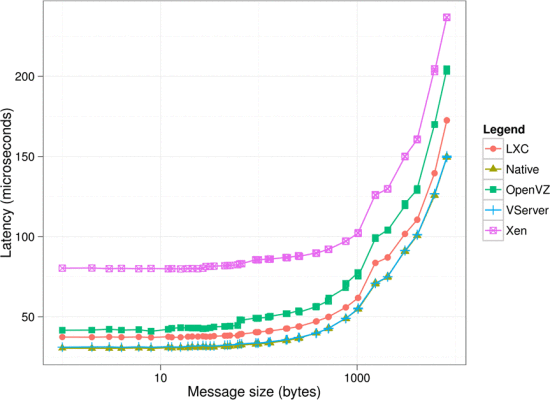
\includegraphics[width=.35\textwidth]{pics/container-delay}
    \caption{Network latency among containers\cite{b8}}
\end{figure}


\subsubsection{Optimizing Container Images}
It can help reduce latency by reducing the amount of loaded data into memory.
This can be done by removing unnecessary files, libraries and
dependencies from the container image.

The study \cite{b29} has shown that optimizing container images by removing unnecessary dependencies and
files results in a 75\% reduction in image size, and the startup time of the optimized
container is 35\% faster than before.

The researchers also found that using a single container with multiple services reduced
startup time by around 50\% compared to using multiple small containers.\cite{b29}


\subsubsection{Using a High-performance Storage Driver}
Using a higher number of container instances per host can improve I/O performance.
Sandro Keil compared the performance of different storage drivers in Docker containers \cite{b30} and
found that OverlayFS has the lowest overhead and fastest performance compared to other
storage drivers\cite{b30,b31,b32}.

In other words, one could use the high-performance storage driver to improve
I/O performance and reduce latency. The number of container instances per host also
has an impact on I/O performance, and increasing the number of container instances may improve
overall I/O throughput. However, this can also lead to increased resource contention and potential
performance degradation if resources are allocated incorrectly.


\subsubsection{Using Host Networking}
Anderson et al.\cite{b33} compared the performance of host networking and container networking in Docker
containers and found that host networking had lower latency and higher throughput. They also
found that using a higher number of containers per host resulted in lower throughput and higher latency.

Using host networking helps reduce latency by allowing containers to use the host's network
interfaces directly\cite{b34,b35}. The reason is that when a container uses host networking mode, it shares
the network namespace with the host and has direct access to the host's network interfaces.
This eliminates the need for NAT and reduces the overhead associated with routing network traffic
through virtual interfaces, which can reduce network latency and improve network performance.

\subsubsection{Using Resource Limits}
Setting resource limits helps prevent containers from using too many resources and causing delays.

Wang et al.\cite{b36} compared the performance of containers with and without resource limits and found
that setting CPU and memory limits improved performance and reduced latency.
Kozhirbayev et al.\cite{b37} found that using container orchestration tools such as Kubernetes helps
optimize resource usage and reduce latency.


